\chapter{Patrones}
\label{apex:patrones}
\textit{El anexo presenta el desarrollo de patrones aplicados a mInstituto}
\vfill
\minitoc
\cleardoublepage

\section{Cadena de Responsabilidad}
Permite a un objeto enviar un comando sin conocer que objeto o objetos lo recibirán, evitando el acoplamiento entre el que envía y el que recibe una petición. Esto permite el paso del comando a un objeto de la cadena que es parte de una gran estructura. Cada objeto de la cadena podría manejar el comando, pasar el comando al siguiente objeto de la cadena, o las dos cosas. \cite{ref12}

  \begin{figure}[H]
 	\centering
  	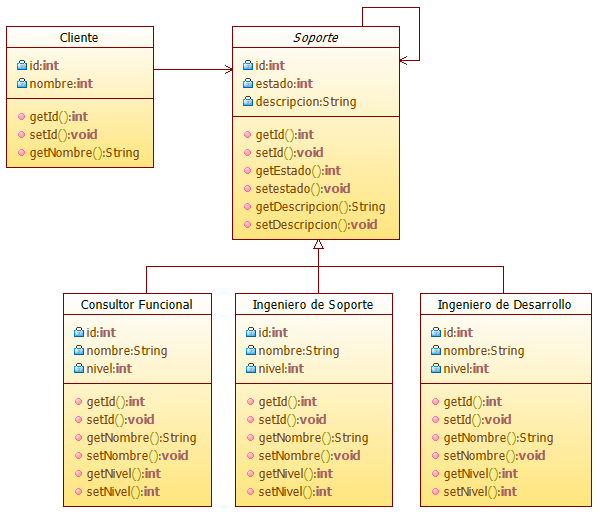
\includegraphics[scale=0.7]{patrones/1}
  	\captionsetup{width=.95\textwidth}
  	\caption{Patrón\index{Patrón} cadena de responsabilidad mInstituto \cite{ref9,ref6}}
  	\label{patron1}
  \end{figure}

  \subsection{Patrón\index{Patrón} cadena de responsabilidad mInstituto}
  Las solicitudes de soporte técnico se pueden manifestar por diferentes medios como el correo electrónico, chat, software de aplicación, y otros más siendo unos de los medios más utilizados el teléfono. Para brindar asistencia a los clientes se ha generalizado la tendencia a la prestación de soporte técnico remoto, donde un técnico se conecta al ordenador mediante una aplicación de conexión remota disminuyendo el tiempo de respuesta, evitando desplazamientos y optimizando varios procesos con esta metodología.
  
  Dependiendo del inconveniente reportado, se pueden dar varios niveles de soporte, donde el soporte nivel 1 es el que está en contacto directo con el usuario y que soluciona las incidencias triviales, soporte nivel 2, daría soporte a las incidencias que no pudieron ser asistidas por el nivel I y el nivel 3, sería la última instancia donde llegarían las incidencias que no fue posible asistir en el nivel II.
  
  El soporte o asistencia técnica está a menudo subdividido en capas, o niveles, para que así pueda atender de una forma más eficaz y eficiente a una base de negocio o clientes. En la empresa se han establecido tres niveles de soporte los cuales son: Consultor funcional, Ingeniero de soporte, Ingeniero de desarrollo.

  \begin{description}
  	\item[Consultor funcional] Nivel 1 de soporte.
  \end{description}
  
  \begin{multicols}{2}[\subsection{Clases cadena de responsabilidad}]
    \lstinputlisting[language=Java,style=java,caption={Cliente.java}]{java/src/Cadena/Cliente.java}
    \lstinputlisting[language=Java,style=java,caption={Soporte.java}]{java/src/Cadena/Soporte.java}
    \lstinputlisting[language=Java,style=java,caption={Consultor.java}]{java/src/Cadena/Consultor.java}
  \end{multicols}
  
\section{Fabrica Abstracta}
Dado un conjunto de clases abstractas relacionadas, el patrón Abstract Factory permite el modo de crear instancias de estas clases abstractas desde el correspondiente conjunto de subclases concretas. Proporciona una interfaz para crear familias de objetos relacionados o dependientes sin especificar su clase concreta. El patrón Abstract Factory puede ser muy útil para permitir a un programa trabajar con una variedad compleja de entidades externas, tales como diferentes sistemas de ventanas con una funcionalidad similar. \cite{ref12}

  \begin{figure}[H]
  	\centering
  	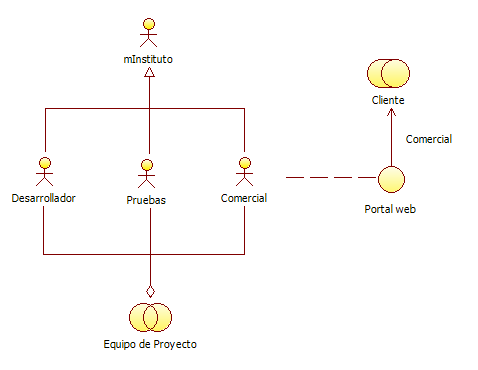
\includegraphics[scale=0.54]{patrones/2}
  	\captionsetup{width=.95\textwidth}
  	\caption{Patrón\index{Patrón} fabrica abstracta mInstituto \cite{ref9,ref6}}
  	\label{patron2}
  \end{figure}
  
  \subsection{Patrón\index{Patrón} Fabrica Abstracta mInstituto}
  La función del contenido original y de calidad a parte de brindar información a nuestros posibles clientes, es la de generar tráfico entrante que generará una mejor posición de nuestro sitio web en los resultados de búsqueda de motores como Google\index{Google}. También hay otros elementos que son igual de importantes como son un diseño responsivo que se puede adaptar a las necesidades del usuario y que le permita trabajar en diferentes dispositivos como su computadora (Portátil) (Windows, Linux\index{Linux}, MacOS), tablet (Ipad) o celular (Iphone, Android\index{Android}, Windows Phone). Sin embargo, es importante que independiente de la vista, el aplicativo tenga un modelo y unos controladores comunes que permitan su funcionalidad en diversas plataformas sin tener que modificar la codificación.
  
  \begin{multicols}{2}[\subsection{Clases fabrica abstracta}]
    \lstinputlisting[language=Java,style=java,caption={Cliente.java}]{java/src/Factory/Cliente.java}
    \lstinputlisting[language=Java,style=java,caption={Ventana.java}]{java/src/Factory/Ventana.java}
    \lstinputlisting[language=Java,style=java,caption={Android.java}]{java/src/Factory/Android.java}
    \lstinputlisting[language=Java,style=java,caption={html.java}]{java/src/Factory/html.java}
    \lstinputlisting[language=Java,style=java,caption={Widget.java}]{java/src/Factory/Widget.java}
    \lstinputlisting[language=Java,style=java,caption={AndroidWidget.java}]{java/src/Factory/AndroidWidget.java}
    \lstinputlisting[language=Java,style=java,caption={MSWidget.java}]{java/src/Factory/MSWidget.java}
    \lstinputlisting[language=Java,style=java,caption={InterfazAbstracta.java}]{java/src/Factory/InterfazAbstracta.java}
    \lstinputlisting[language=Java,style=java,caption={InterfazHTML.java}]{java/src/Factory/InterfazHTML.java}
    \lstinputlisting[language=Java,style=java,caption={InterfazAndroid.java}]{java/src/Factory/InterfazAndroid.java}
  \end{multicols}
  
\section{Decorador}
Extiende la funcionalidad de un objeto dinámicamente de tal modo que es transparente a sus clientes, utilizando una instancia de una subclase de la clase original que delega las operaciones al objeto original. Provee una alternativa muy flexible para agregar funcionalidad a una clase. \cite{ref12}

  \subsubsection{Aplicabilidad}
  \begin{itemize}
  	\item Hay una necesidad de extender la funcionalidad de una clase, pero no hay razones para extenderlo a través de la herencia.
  	\item Hay la necesidad de extender dinámicamente la funcionalidad de un objeto y quizás quitar la funcionalidad extendida.
  \end{itemize}

  \begin{figure}[H]
	\centering
	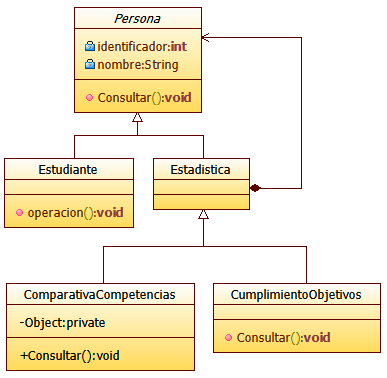
\includegraphics[scale=0.7]{patrones/3}
	\captionsetup{width=.95\textwidth}
	\caption{Patrón\index{Patrón} decorador mInstituto \cite{ref9,ref6}}
	\label{patron2}
  \end{figure}

  \subsection{Patrón\index{Patrón} Decorador mInstituto}
  Con este patrón queremos resaltar la estructura modular característica de minstituto que nos permitirá ir agregando funcionalidades a cada uno de los perfiles del sistema. Para nuestro caso los Estudiantes heredan sus cualidades de la clase persona y se les ira agregando nuevas funcionalidades, una inicial de estadística que luego incrementará su nivel de complejidad o detalle a medida que se desarrollan las actividades y objetivos permitiendo que puedan generar comparativas con sus compañeros y podrán verificar el nivel de cumplimento de objetivos en la institución.

\begin{multicols}{2}[\subsection{Clases Decorador}]
	\lstinputlisting[language=Java,style=java,caption={Persona.java}]{java/src/Decorator/Persona.java}
	\lstinputlisting[language=Java,style=java,caption={Estudiante.java}]{java/src/Decorator/Estudiante.java}
	\lstinputlisting[language=Java,style=java,caption={Estadistica.java}]{java/src/Decorator/Estadistica.java}
	\lstinputlisting[language=Java,style=java,caption={ComparativaCompetencias.java}]{java/src/Decorator/ComparativaCompetencias.java}
	\lstinputlisting[language=Java,style=java,caption={CumplimientoObjetivos.java}]{java/src/Decorator/CumplimientoObjetivos.java}
\end{multicols}

\chapter{Resumen Simbología\index{Simbología} Archimate\index{Archimate} 2.1}
\label{apex:anexos}
\textit{El presente anexo describe la Simbología\index{Simbología} de Archimate\index{Archimate} utilizada como referencia en el modelamiento de la Arquitectura Empresarial\index{Arquitectura Empresarial}.}
\vfill
\minitoc
\cleardoublepage

\section{Capa de Negocio\index{Negocio}s}
  \begin{longtable}
	{m{3cm}m{4.8cm}m{5.2cm}}
	\hline
	\rowcolor[HTML]{0073a1}
	{\color[HTML]{FFFFFF} \textbf{Concepto}} & {\color[HTML]{FFFFFF} \textbf{Definición}} & {\color[HTML]{FFFFFF} \textbf{Notación}} \\
	\hline
	 Actor & Una entidad de organización que es capaz de realizar la conducta a través de un rol. & 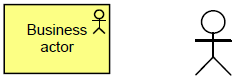
\includegraphics[scale=0.5]{figuras/36} \\ \hline
	 Role & La responsabilidad de llevar a cabo un comportamiento específico, al que se le puede asignar un actor. & 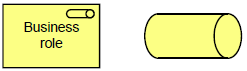
\includegraphics[scale=0.5]{figuras/37} \\ \hline
	 Colaboración\index{Colaboración} & Un agregado de dos o más funciones de negocios que trabajan en conjunto para llevar a cabo el comportamiento colectivo. & 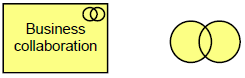
\includegraphics[scale=0.5]{figuras/38} \\ \hline
	 Interface\index{Interface} & Un punto de acceso donde se pone a disposición un servicio de negocio al entorno. & 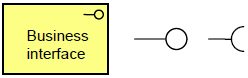
\includegraphics[scale=0.5]{figuras/39} \\ \hline
	 Localización & Un punto conceptual o extensión en el espacio. & 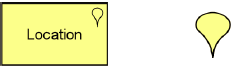
\includegraphics[scale=0.5]{figuras/40} \\ \hline
	 Proceso\index{Proceso} & Un elemento de la conducta que el comportamiento de los grupos basa en un ordenamiento de las actividades. Se tiene la intención de producir un conjunto definido de productos o servicios. & 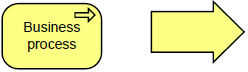
\includegraphics[scale=0.5]{figuras/41} \\ \hline
	 Función & Un elemento de la conducta que el comportamiento de los grupos basada en una seleccion en un conjunto seleccionado de criterios (recursos empresariales suelen ser necesarios y / o competencias). & 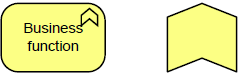
\includegraphics[scale=0.5]{figuras/42} \\ \hline
	 Interacción & Un elemento de comportamiento que describe el comportamiento de una colaboración de negocios. & 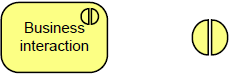
\includegraphics[scale=0.5]{figuras/43} \\ \hline
	 Evento & Algo que sucede (interna o externa) e influye en el comportamiento (de negocios proceso, la función empresarial, la interacción de negocios). & 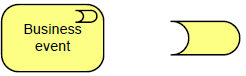
\includegraphics[scale=0.5]{figuras/44} \\ \hline
	 Servicio\index{Servicio} & Un servicio que satisface una necesidad comercial de un cliente (interno o externo a la organización). & 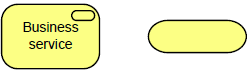
\includegraphics[scale=0.5]{figuras/45} \\ \hline
	 Objeto & Un elemento pasivo que tiene relevancia desde un punto de vista comercial. & 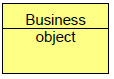
\includegraphics[scale=0.5]{figuras/46} \\ \hline
	 Representación & Una forma perceptible de la información transportada por un objeto de negocio. & 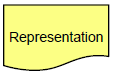
\includegraphics[scale=0.5]{figuras/47} \\ \hline
	 Sentido & El conocimiento o experiencia presente en un objeto de negocio o de su representación, dado un contexto particular. & 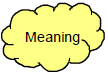
\includegraphics[scale=0.5]{figuras/48} \\ \hline
	 Valor & El valor relativo, utilidad o importancia de un servicio de negocio o producto. & 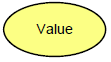
\includegraphics[scale=0.5]{figuras/49} \\ \hline
	 Producto\index{Producto} & Una colección coherente de los servicios, acompañada de un contrato / conjunto de acuerdos, que se ofrece en su conjunto a los clientes (internos o externos). & 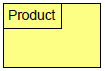
\includegraphics[scale=0.5]{figuras/50} \\ \hline
	 Contrato & Una especificación formal o informal de acuerdo que especifica los derechos y obligaciones inherentes a un producto. & 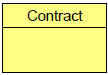
\includegraphics[scale=0.5]{figuras/51} \\
	\bottomrule
    \captionsetup{width=.95\textwidth}
    \caption{Simbología\index{Simbología} capa de Negocio\index{Negocio}s \cite{ref9}}
    \label{tabla29}
  \end{longtable}

\newpage
\section{Capa de Aplicación\index{Aplicación}}
  \begin{longtable}
  	{m{3cm}m{4.8cm}m{5.2cm}}
  	\hline
  	\rowcolor[HTML]{0073a1}
  	{\color[HTML]{FFFFFF} \textbf{Concepto}} & {\color[HTML]{FFFFFF} \textbf{Definición}} & {\color[HTML]{FFFFFF} \textbf{Notación}} \\
  	\hline
	Componente & Parte modular, desplegable, y reemplazable de un sistema de software que encapsula su comportamiento y los datos y expone a estos a través de un conjunto de interfaces. & 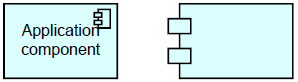
\includegraphics[scale=0.5]{figuras/52} \\ \hline
	Colaboración\index{Colaboración} & Un agregado de dos o más componentes de aplicaciones que funcionan en conjunto para llevar a cabo el comportamiento colectivo. & 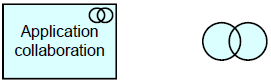
\includegraphics[scale=0.5]{figuras/53} \\ \hline
	Interface\index{Interface}s & Un punto de acceso donde se pone a disposición un servicio de aplicaciones para un usuario u otro componente de la aplicación. & 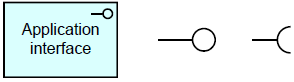
\includegraphics[scale=0.5]{figuras/54} \\ \hline
	Función & Un elemento de comportamiento que los grupos de comportamiento que puede ser realizada por un componente de aplicación automatizado. & 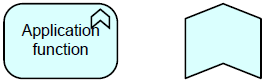
\includegraphics[scale=0.5]{figuras/55} \\ \hline
	Interacción & Un elemento de comportamiento que describe el comportamiento de una aplicación colaborativa. & 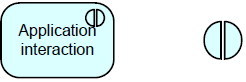
\includegraphics[scale=0.5]{figuras/56} \\ \hline
	Servicio\index{Servicio} & Un servicio que expone comportamiento automatizado. & 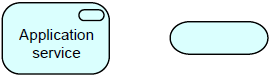
\includegraphics[scale=0.5]{figuras/57} \\ \hline
	Objeto & Un elemento pasivo que permite su tratamiento automatizado. & 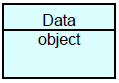
\includegraphics[scale=0.5]{figuras/58} \\
	\bottomrule
	\captionsetup{width=.95\textwidth}
	\caption{Simbología\index{Simbología} capa de Aplicación\index{Aplicación} \cite{ref9}}
	\label{tabla30}
  \end{longtable}

\newpage
\section{Capa de Tecnología\index{Tecnología}}
  \begin{longtable}
  	{m{3cm}m{4.8cm}m{5.2cm}}
  	\hline
  	\rowcolor[HTML]{0073a1}
  	{\color[HTML]{FFFFFF} \textbf{Concepto}} & {\color[HTML]{FFFFFF} \textbf{Definición}} & {\color[HTML]{FFFFFF} \textbf{Notación}} \\
  	\hline
	Nodo & Un recurso computacional sobre los que los artefactos se pueden almacenar o desplegar para su ejecución. & 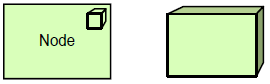
\includegraphics[scale=0.5]{figuras/59} \\ \hline
	Dispositivo & Un recurso de hardware sobre el cual los artefactos se pueden almacenar o desplegar para su ejecución. & 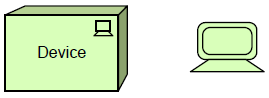
\includegraphics[scale=0.5]{figuras/60} \\ \hline
	Red & Un medio de comunicación entre dos o más dispositivos. & 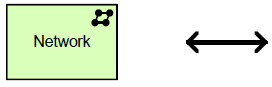
\includegraphics[scale=0.5]{figuras/61} \\ \hline
	Ruta comunicación & Un enlace entre dos o más nodos, a través del cual estos pueden intercambiar datos. & 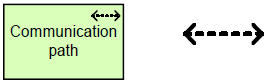
\includegraphics[scale=0.5]{figuras/62} \\ \hline
	Infraestructura\index{Infraestructura} & Un punto de acceso en caso de los servicios de infraestructura ofrecidos por un nodo puede acceder a otros nodos y componentes de la aplicación. & 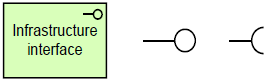
\includegraphics[scale=0.5]{figuras/63} \\ \hline
	Software\index{Software} & Un entorno de software para los tipos específicos de componentes y objetos que se despliegan en ella en forma de artefactos. & 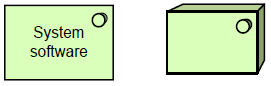
\includegraphics[scale=0.5]{figuras/64} \\ \hline
	Función & Un elemento de comportamiento que agrupa infraestructura. Comportamiento\index{Comportamiento} que puede ser realizado por un nodo. & 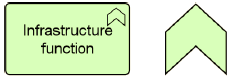
\includegraphics[scale=0.5]{figuras/65} \\ \hline
	Servicio\index{Servicio} & Una unidad externa visible de la funcionalidad proporcionada por uno o más nodos, expuesta a través de interfaces bien definidas, y significativo para el entorno. & 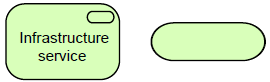
\includegraphics[scale=0.5]{figuras/66} \\ \hline
	Artefacto\index{Artefacto} & Una pieza física de datos que se utilizan o producen en un proceso de desarrollo de software, o por la implementación y operación de un sistema. & 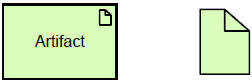
\includegraphics[scale=0.5]{figuras/67} \\
	\bottomrule
	\captionsetup{width=.95\textwidth}
	\caption{Simbología\index{Simbología} capa de Tecnología\index{Tecnología} \cite{ref9}}
	\label{tabla31}
  \end{longtable}
  
\section{Relaciones}
  \subsection{Estructura\index{Estructura}les}
    \begin{longtable}
    	{m{3cm}m{4.8cm}m{5.2cm}}
    	\hline
    	\rowcolor[HTML]{0073a1}
    	{\color[HTML]{FFFFFF} \textbf{Concepto}} & {\color[HTML]{FFFFFF} \textbf{Definición}} & {\color[HTML]{FFFFFF} \textbf{Notación}} \\
    	\hline
    	Asociación & Los modelos de asociación de una relación entre los objetos que no está cubierta por otro, la relación más específica. & 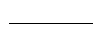
\includegraphics[scale=0.5]{figuras/68} \\ \hline
    	Acceso & La relaciones de acceso en los modelos unen los conceptos de comportamiento a los objetos de negocio o de datos. & 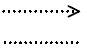
\includegraphics[scale=0.5]{figuras/69} \\ \hline
    	Usado por & La relación de uso une los servicios por parte de los procesos, funciones o las interacciones y el acceso a las interfaces de funciones, componentes o colaboraciones. & 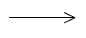
\includegraphics[scale=0.5]{figuras/70} \\ \hline
    	Realización & La relación realización vincula a una entidad lógica con una entidad más concreta que se da cuenta de ello. & 
\includegraphics[scale=0.5]{figuras/71} \\ \hline
    	Asignación\index{Asignación} & La relación de asignación vincula unidades de comportamiento con los elementos activos (por ejemplo, funciones, componentes) que las llevan a cabo, o roles con actores que las cumplen. & 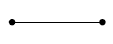
\includegraphics[scale=0.5]{figuras/72} \\ \hline
    	Agregación & La relación de agregación indica que un grupo de objetos es una serie de otros objetos. & 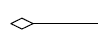
\includegraphics[scale=0.5]{figuras/73} \\ \hline
    	Composición\index{Composición} & La relación composición indica que un objeto está compuesto por uno o más de otros objetos. & 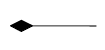
\includegraphics[scale=0.5]{figuras/74} \\
  	    \bottomrule
    	\captionsetup{width=.95\textwidth}
    	\caption{Simbología\index{Simbología} de Relaciones Estructura\index{Estructura}les \cite{ref9}}
    	\label{tabla32}
    \end{longtable}
    
    \subsection{Dinámicas}
        \begin{longtable}
        	{m{3cm}m{4.8cm}m{5.2cm}}
        	\hline
        	\rowcolor[HTML]{0073a1}
        	{\color[HTML]{FFFFFF} \textbf{Concepto}} & {\color[HTML]{FFFFFF} \textbf{Definición}} & {\color[HTML]{FFFFFF} \textbf{Notación}} \\
        	\hline
        	Flujo & La relación de flujo describe el intercambio o de transferencia, por ejemplo, la información o el valor entre los procesos, funciones, interacciones y eventos. & 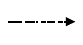
\includegraphics[scale=0.5]{figuras/75} \\ \hline
        	Disparo & La relación de disparo describe las relaciones temporales o causales entre procesos, funciones, interacciones y eventos. & 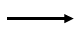
\includegraphics[scale=0.5]{figuras/76} \\
   	  	    \bottomrule
  	  	    \captionsetup{width=.95\textwidth}
   	  	    \caption{Simbología\index{Simbología} de Relaciones Dinámicas \cite{ref9}}
   	  	    \label{tabla33}
   	  	\end{longtable}
   	  	
  	    \subsection{Otras}
    	    \begin{longtable}
    	    	{m{3cm}m{4.8cm}m{5.2cm}}
    	    	\hline
    	    	\rowcolor[HTML]{0073a1}
    	    	{\color[HTML]{FFFFFF} \textbf{Concepto}} & {\color[HTML]{FFFFFF} \textbf{Definición}} & {\color[HTML]{FFFFFF} \textbf{Notación}} \\
    	    	\hline
   	  	    	Grupo & La relación indica que la agrupación de objetos del mismo tipo o de tipos diferentes, uno para el otro basado en alguna característica común. & 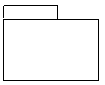
\includegraphics[scale=0.5]{figuras/77} \\ \hline
   	  	    	Unión & Una unión se utiliza para conectar las relaciones del mismo tipo. & 
\includegraphics[scale=0.5]{figuras/78} \\ \hline
   	  	    	Especialización\index{Especialización} & La relación especialización indica que un objeto es una especialización de otro objeto. & 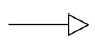
\includegraphics[scale=0.5]{figuras/79} \\
   	  	    	\bottomrule
   	  	    	\captionsetup{width=.95\textwidth}
   	  	    	\caption{Simbología\index{Simbología} de otras Relaciones \cite{ref9}}
   	  	    	\label{tabla34}
   	  	    \end{longtable}
   	  	    
\section{Motivación}
  \begin{longtable}
  	{m{3cm}m{4.8cm}m{5.2cm}}
  	\hline
  	\rowcolor[HTML]{0073a1}
  	{\color[HTML]{FFFFFF} \textbf{Concepto}} & {\color[HTML]{FFFFFF} \textbf{Definición}} & {\color[HTML]{FFFFFF} \textbf{Notación}} \\
  	\hline
  	Stakeholder\index{Stakeholder} & El papel de un individuo, equipo u organización (o clases de los mismos) que representa sus intereses en, o preocupaciones en relación con, el resultado de la arquitectura. & 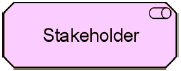
\includegraphics[scale=0.5]{figuras/80} \\ \hline
  	Manejador\index{Manejador} & Algo que crea, motiva y alimenta el cambio en una organización. & 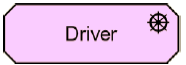
\includegraphics[scale=0.5]{figuras/81} \\ \hline
  	Valoración & El resultado de un análisis de algún conductor. & 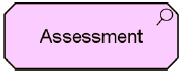
\includegraphics[scale=0.5]{figuras/82} \\ \hline
  	Objetivo & Un estado final de que una parte interesada tiene la intención de lograr. & \includegraphics[scale=0.5]{figuras/83} \\ \hline
  	Requerimiento & Una declaración de necesidad que debe ser realizado por un sistema. & \includegraphics[scale=0.5]{figuras/84} \\ \hline
  	Restricción & Una restricción en el modo en que se realiza un sistema. & \includegraphics[scale=0.5]{figuras/85} \\ \hline
  	Principio\index{Principio} & Una propiedad normativo de todos los sistemas en un contexto dado, o la forma en que se realizan. & \includegraphics[scale=0.5]{figuras/86} \\
	\bottomrule
	\captionsetup{width=.95\textwidth}
	\caption{Simbología\index{Simbología} capa de Motivación \cite{ref9}}
	\label{tabla35}
  \end{longtable}

\newpage
\section{Implementación\index{Implementación} y Migración\index{Migración}}
  \begin{longtable}
  	{m{3cm}m{4.8cm}m{5.2cm}}
  	\hline
  	\rowcolor[HTML]{0073a1}
  	{\color[HTML]{FFFFFF} \textbf{Concepto}} & {\color[HTML]{FFFFFF} \textbf{Definición}} & {\color[HTML]{FFFFFF} \textbf{Notación}} \\
  	\hline
	Paquete de trabajo & Una serie de acciones destinadas a lograr un objetivo único dentro de un tiempo especificado. & \includegraphics[scale=0.5]{figuras/87} \\ \hline
	Entregable & Un resultado definido con precisión de un paquete de trabajo. & \includegraphics[scale=0.5]{figuras/88} \\ \hline
	Platea & Un estado relativamente estable de la arquitectura que existió durante un período de tiempo limitado. & \includegraphics[scale=0.5]{figuras/89} \\ \hline
	Brecha & Uno de los resultados de un análisis de la brecha entre dos plateas. & \includegraphics[scale=0.5]{figuras/90} \\
	\bottomrule
	\captionsetup{width=.95\textwidth}
	\caption{Simbología\index{Simbología} capa de Implementación\index{Implementación} y Migración\index{Migración} \cite{ref9}}
	\label{tabla36}
  \end{longtable}
  
%\chapter{A Software\index{Software} Architecture Proposal Artistic Engineering Environment -AEE}
%\label{apex:articulo}
%\textit{El presente anexo describe la Simbología\index{Simbología} de Archimate\index{Archimate} utilizada como referencia en el modelamiento de la Arquitectura Empresarial\index{Arquitectura Empresarial}. El siguiente anexo corresponde a una Publicación utilizada como referencia relevante para el desarrollo del proyecto de grado.}
%\vfill
%\cleardoublepage
%\includepdf[pages=-]{pdfs/AIA.pdf}